% Chapter 1
\chapter{Marco Teórico} % Main chapter title

\label{Cap_SDT} % For referencing the chapter elsewhere, use \ref{Chapter1} 

%----------------------------------------------------------------------------------------

% Define some commands to keep the formatting separated from the content 
\newcommand{\keyword}[1]{\textbf{#1}}
\newcommand{\tabhead}[1]{\textbf{#1}}
\newcommand{\code}[1]{\texttt{#1}}
\newcommand{\file}[1]{\texttt{\bfseries#1}}
\newcommand{\option}[1]{\texttt{\itshape#1}}

%----------------------------------------------------------------------------------------

\section{Teoría de Detección de Señales}

%Detectar ciertos estados en el mundo es importante para guiar nuestro comportamiento
Uno de los problemas más frecuentes a los que se enfrentan los organismos como sistemas inmersos en entornos variables que buscan optimizar su comportamiento, es la detección de estados o eventos específicos -señales- que de acuerdo a su experiencia y tras la definición de ciertas relaciones de contingencia, les proporcionen información relevante sobre el estado del mundo, las restricciones vigentes y la disponibilidad de eventos biológicamente importantes.\\

%Origen y expansión de la Teoría de Detección de Señales en la psicología y otras áreas
La Teoría de Detección de Señales (TDS o SDT, por sus siglas en inglés) aparece por primera vez en 1954 -como tantos otros avances científicos y tecnológicos motivados por las necesidades planteadas por la Segunda Guerra Mundial- en el contexto del estudio y desarrollo de radares para detectar señales eléctricas específicas \parencite{Peterson1954}. Muy poco tiempo después, los psicólogos John A. Swets y Wilson P. Tanner contribuyeron a la expansión de la teoría a un contexto psicológico, como un modelo para estudiar la percepción de los organismos, \parencite{Tanner1954, Swets1961}. Desde entonces, la TDS constituye uno de los modelos más estudiados, desarrollados y ampliamente aplicados en Psicología, extendiéndose desde su foco inicial en el estudio de la percepción \parencite{Rosenholtz2001, Pessoa2005, Wallis2007} hacia el estudio de cualquier fenómeno o tarea donde los organismos se enfrenten al problema de emitir -y guiar su comportamiento en función a- juicios de detección; por ejemplo, en materia de la emisión de diagnósticos clínicos \parencite{Grossberg1978, Swets2000, Boutis2010}, en el estudio de ciertas condiciones clínicas \parencite{Westermann2010, Bonnel2003, Brown1994, Naliboff1981}, en el estudio de la identificación visual de testigos \parencite{Gronlund2014, Wixted2014, Wixted2016} y un muy amplio 'etcétera' \parencite{Gordon1974, Nuechterlein1983, Harvey1992, Verghese2001}.\\ 

%La Teoría de Detección de señales como un modelo descriptivo para el problema de la detección que admite la importancia de la incertidumbre, como parte del entorno y como motor en el uso de sesgos de respuesta.
La TDS constituye un modelo estadístico que describe el problema al que se enfrentan los organismos inmersos en situaciones de detección en ambientes con incertidumbre, donde las señales -los estímulos cuya ocurrencia interesa detectar- coexisten con ruido -estímulos que no son la señal pero que pueden confundirse con esta-. Se trata de un modelo de decisión que entiende la detección como una tarea de elección, donde los organismos no responden simplemente con base en lo que perciben, sino que eligen el juicio de detección que les permita guiar su comportamiento de la manera mas óptima posible dada la información que poseen y la evidencia presente.\\

La generalizabilidad del modelo de la TDS al estudio de distintos fenómenos y tareas de detección se debe a lo abstracto de sus elementos: la 'señal' que interesa detectar puede ser desde un estímulo concreto -una luz o un tono- hasta la pertenencia a una categoría -una enfermedad o amenaza- y el 'ruido' es simplemente todo elemento presente en el entorno de la tarea que no sea la señal.\\ 

\subsection{Supuestos generales del modelo}

%La TDS distingue dos grandes factores en la emisión de un juicio o respuesta: La discriminabilidad y el sesgo.
La TDS funciona como una herramienta -o marco de análisis- para traducir el desempeño observado en tareas de detección en inferencias sobre la precisión con que la señal se distingue del ruido (la discriminabilidad) y la posible preferencia -o tendencia- del sistema detector a responder en favor o en contra de esta (el sesgo). Esta distinción entre la Discriminabilidad de los estímulos comprometidos y el Sesgo del sistema, como factores que interactúan en la emisión de juicios de detección, es una de las principales propiedades de la TDS cuya importancia e implicaciones se discuten a continuación:\\

\textbf{1.- El papel de la Discriminabilidad: Siempre hay incertidumbre}\\

%Hay variabilidad en todos los estímulos implicados en las tareas de detección (en la señal y en los estímulos no-señal)
Se habla de la detección de señales como un problema de adaptación porque se asume que la variabilidad en la presentación y percepción de los estímulos en el ambiente merma la capacidad de los organismos de emitir juicios de detección que reflejen el estado del mundo con certeza. Y dado que los estímulos-señal coexisten en el mundo con estímulos-ruido, saber qué tan salientes son las señales respecto del ruido es uno de los factores más importantes para determinar qué tan difícil es su detección para los organismos. En términos de la TDS, se habla de dicha dificultad como 'la discriminabilidad' de los estímulos comprometidos en la tarea.\\

De acuerdo con la TDS, la discriminabilidad constituye el primer gran componente en la emisión de juicios de detección óptimos que reflejen el verdadero estado del mundo y permitan al organismo actuar conforme a las consecuencias vigetes. Suele explicarse en términos de:\\ %  1) la variabilidad intrínseca en la presentación de las señales y 2) el ruido con que ésta coexiste.\\

\underline{a) La Variabilidad en la Señal}\\

%Existe variabilidad en la forma en que percibimos los estímulos que nos rodean. Los sistemas sensoriales y perceptuales se comportan como instrumentos de medición (error de medida)
La noción de variabilidad ha sido uno de los principales motores para el desarrollo de modelos estadísticos en Psicología. Desde que Fechner extendiera las ideas planteadas por Gauss sobre la incertidumbre contenida en toda medición -la idea de que toda medición realizada contiene el valor 'verdadero' de aquello que se quiere medir más un 'error' aleatorio que la carga de incertidumbre- al estudio de la percepción -conceptualizando nuestros sistemas sensoriales y perceptuales como 'instrumentos de medición' que perciben las cualidades 'verdaderas' de los estímulos más un 'error' en cada observación- \parencite{Fechner, Gauss}, se sentaron las bases para el desarrollo de una amplia gama de modelos matemáticos y estadísticos en Psicofísica orientados a estudiar la relación entre las cualidades físicas -'reales'- de los estímulos y la magnitud o intensidad con que se perciben psicológicamente \parencite{Link1994}.\\

%Variabilidad en la percepción de un mismo estímulo.
En el marco de la TDS, la variabilidad se considera una propiedad intrínseca de las señales a detectar bajo el supuesto de que ningún estímulo se percibe o se presenta de manera idéntica en cada exposición. Por ejemplo, imaginemos los siguientes casos: \\

\begin{itemize}
	\item Una persona es expuesta a un mismo tono con intensidad X en cien ocasiones distintas y tras cada presentación, asigna un valor a la intensidad percibida. El valor reportado en cada ensayo será una mezcla entre el valor real del tono y un error aleatorio. Como se muestra en la Figura~\ref{fig:Senal_percepcion}, es muy probable que el valor percibido y reportado coincida con -o se acerque bastante a- su valor real (la media de la distribución, $\mu$, señalada con una línea vertical roja), pero también habrá ensayos en que aún tratándose del mismo estímulo, el valor percibido caiga por encima o por debajo de su valor real con cierta dispersión (las colas de la distribución). Es decir, existe variabilidad en la forma en que se perciben los estímulos.\\

	\item Un psicólogo aplica una prueba clínica 'A' para evaluar si su paciente tiene depresión. Por lo general, las pruebas clínicas arrojan un puntaje 'p' que, de acuerdo a su correspondencia con el rango de puntajes típicamente obtenidos por personas que tienen la condición, sugieren qué diagnóstico emitir. La Figura~\ref{fig:Senal_presentacion} presenta la idea central de este ejemplo: no todas las personas con depresión obtienen exactamente el mismo puntaje, sino que dentro de la serie de posibles puntajes a obtener en la prueba (todos los valores en el eje de las x), las personas con depresión suelen obtener resultados dentro de un rango específico con cierta probabilidad (la distribución azul), de tal suerte que hay puntajes que se asocian con dicha condición con mayor probabilidad (siendo la media de la distribución, $\mu$, señalada en rojo la más probable) que otros. En otras palabras, hay variabilidad en la presentación de ciertos estímulos en el entorno.\\
\end{itemize}

\begin{figure}[th]
\centering
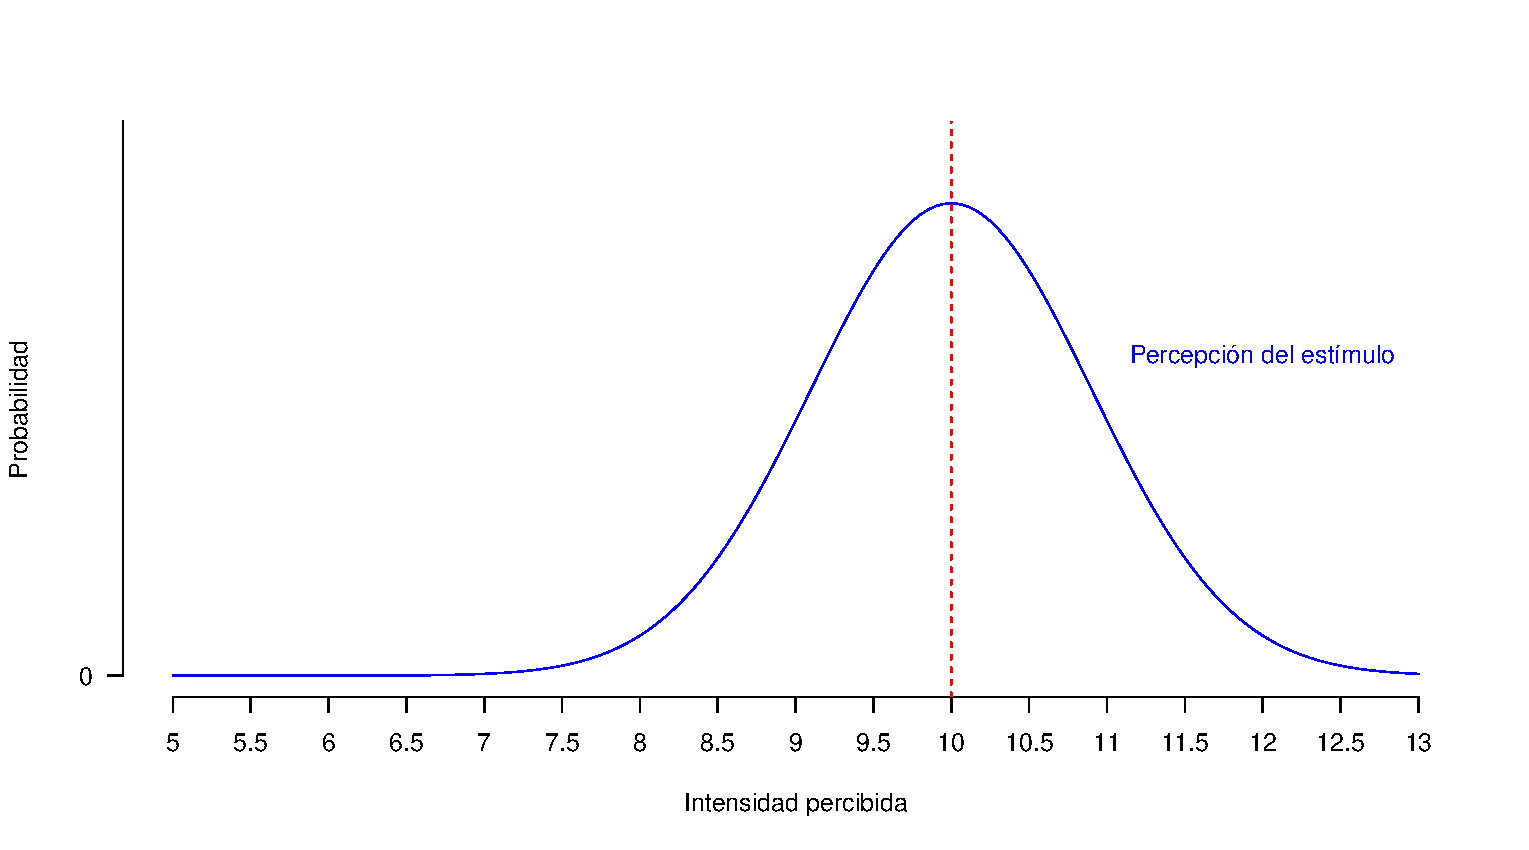
\includegraphics[width=0.80\textwidth]{Figures/Signal_Perception} 
%\decoRule
\caption[Variabilidad en la percepción de los estímulos]{Figura representativa de la variabilidad en la percepción de los estímulos. Si se presenta un mismo estímulo con intensidad x en repetidas ocasiones, es muy probable que el valor percibido se acerque a su valor real, (la media de la distribución, $\mu$) sin embargo y aunque con menor probabilidad, también habrán ocasiones en que sea percibido como más, o menos, intenso, (siendo cada vez menos probables conforme se alejan del valor 'real'.}
\label{fig:Senal_percepcion}
\end{figure}


\begin{figure}[th]
\centering
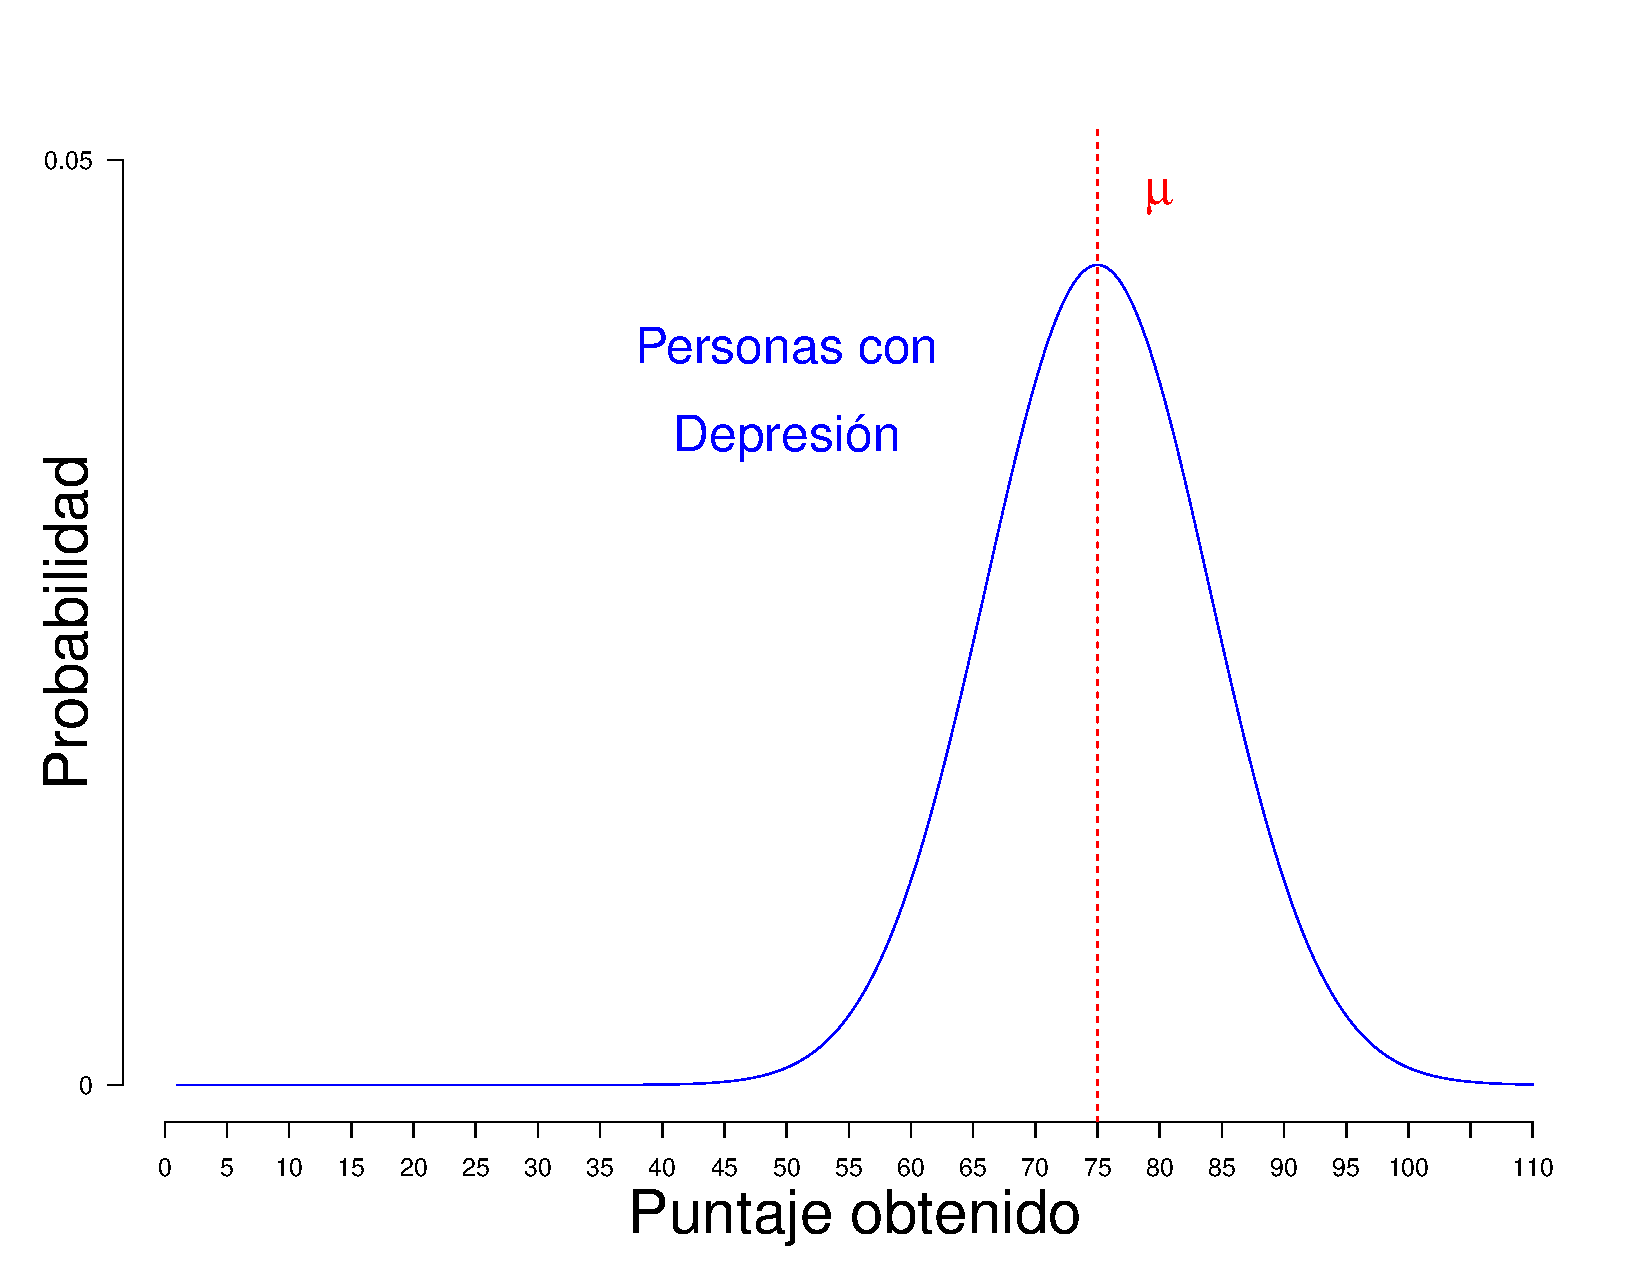
\includegraphics[width=0.80\textwidth]{Figures/Signal_Presentation} 
%\decoRule
\caption[Variabilidad en la presentación de los estímulos]{Figura representativa de la variabilidad en la presentación de los estímulos. Al aplicar una prueba clínica para detectar casos de Depresión, el diagnóstico emitido a partir de los puntajes observados se hace en relación a un rango identificado de valores que se asocian a dicha condición con mayor o menor probabilidad al rededor de una media ($\mu$, señalado en rojo). Los valores representados son arbitrarios.}
\label{fig:Senal_presentacion}
\end{figure}


En general, las Figuras~\ref{fig:Senal_percepcion} y \ref{fig:Senal_presentacion} representan un elemento fundamental para la forma en que la TDS concibe la detección de señales como un problema de adaptabilidad: la variabilidad es intrínseca a la presentación de los estímulos, ya sea porque nuestros sistemas sensoriales no los capturan igual en cada presentación, o porque los estímulos no se nos presentan exactamente de la misma forma en cada ocasión. Es decir, los estímulos en cuya detección están interesados los organismos (las señales) son variables en sí mismos.\\

    \underline{b) La variabilidad en el Entorno: Ruido}\\

%La señal coexiste con el ruido y puede llegar a confundirse con el mismo.
Además del hecho de que existe variabilidad implícita en las señales a detectar, es necesario tomar en cuenta que estas coexisten en el mundo con otros estímulos o estados que -dada su propia variabilidad- pueden llegar a producir evidencia similar y confundir el diagnóstico de detección emitido por los organismos implicados en la tarea.\\

Retomando el ejemplo planteado en la Figura~\ref{fig:Senal_presentacion} acerca de la variabilidad en los puntajes observados en personas con una condición particular en una prueba clínica, la Figura~\ref{fig:Noise} ilustra por añadidura un segundo punto clave para entender por qué se habla de la detección de señales como un problema con incertidumbre. Ya que así como las personas con depresión no obtienen siempre un mismo puntaje, no todas las personas que presentan la prueba sin tener la condición obtienen un cero absoluto -o cualquier otro puntaje fijo- como resultado, sino que a su vez obtienen puntajes dentro de su propia distribución de probabilidad (la distribución agregada en color negro). Nótese que existe un pequeño conjunto de valores a lo largo de los cuales se traslapan las dos distribuciones y tomemos en cuenta que las evaluaciones clínicas se realizan para detectar -diagnosticar- cierta condición en la persona evaluada -la señal- de acuerdo al resultado obtenido; ¿Cuál sería el diagnóstico pertinente para una persona que obtuvo 63 puntos en la prueba? Parece ser que dicha evidencia corresponde con lo observado tanto en los casos que contienen la señal, como en los que no. Sin embargo, dentro de este rango compartido de puntajes a observar en personas con o sin depresión, parece ser que existen algunos (los más cercanos a la media de la distribución de señal) que son más probables en personas con dicha condición, y viceversa. Sin embargo, el punto es claro: existe incertidumbre en la tarea en tanto que la señal y el ruido pueden llegar a producir la misma evidencia.\\ 

\begin{figure}[th]
\centering
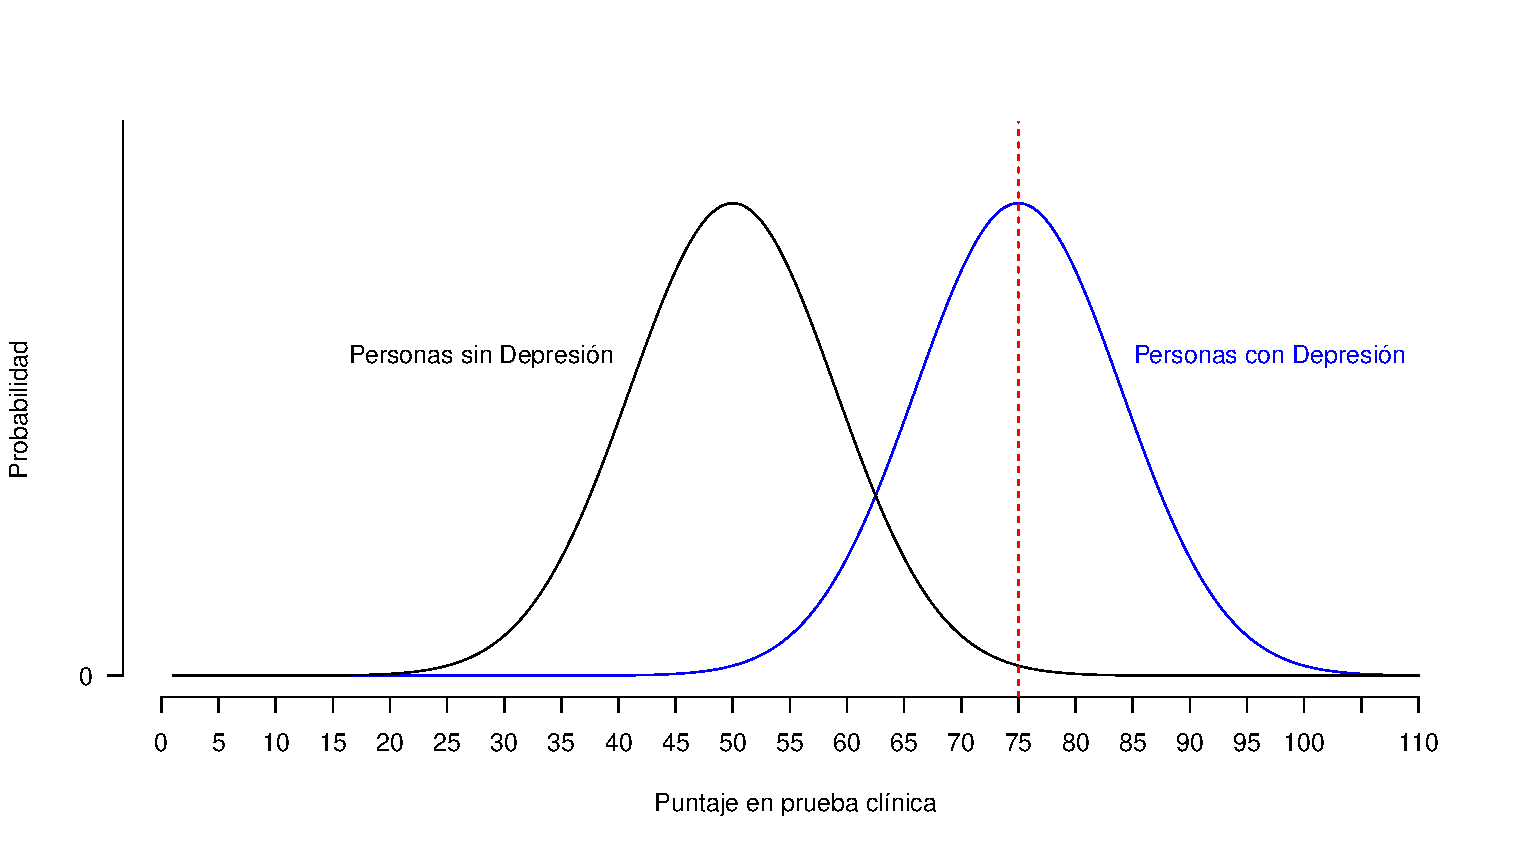
\includegraphics[width=0.80\textwidth]{Figures/Noise} 
%\decoRule
\caption[Variabilidad en la señal y en el ruido]{Extensión del ejemplo acerca de la aplicación de una prueba clínica para detectar casos de depresión. Se presenta una distribución para representa el rango de puntajes asociados con dicha condición (en azul) y se agrega una nueva distribución que representa el rango de puntajes observados en personas sin depresión que realizan esta misma prueba (en negro). La Figura ilustra la noción de que los posibles estados de mundo -señal y ruido- se presentan y perciben dentro de su propia variabilidad en cada ocasión, siendo posible que la evidencia producida se confunda entre sí. Los valores utilizados son arbitrarios.}
\label{fig:Noise}
\end{figure}

Al hablar de Discriminabilidad en tareas de detección bajo el marco de la TDS, se hace referencia a la probabilidad con que la señal y el ruido producen la misma evidencia (o bien, "¿qué tan probable es que la señal y el ruido se confundan?"). Y en términos de la representación gráfica del problema con sus respectivas distribuciones de probabilidad, implica una evaluación de qué tan grande es el área de sobrelape, al considerar esta un indicador fundamental de la incertidumbre contenida en la tarea ("¿Qué tan discriminable -diferente- es la señal respecto del ruido?").\\

La Figura~\ref{fig:Overlap} presenta dos figuras representativas que ilustran la relación entre la distancia entre las distribuciones de ruido y señal, el área de sobrelape entre estas y su interpretación en términos de la discriminabilidad de los estímulos contenidos en la tarea. En el panel superior (a), las distribuciones están muy separadas y el sobrelape entre estas es pequeño, sugiriendo un entorno con poca incertidumbre donde es muy poco probable encontrar evidencia que pueda confundir al organismo entre ambos estados del mundo -discriminabilidad alta-. Por otro lado, si las distribuciones están más juntas, como ocurre en el panel inferior (b), el sobrelape será cada vez mayor, indicando que existe un rango amplio de valores-evidencia vinculados simultáneamente con ambos estados del mundo y ante los cuales el organismo no podría tener certeza sobre a cuál de estos adjudicar su observación -discriminabilidad baja-.\\

\begin{figure}[th]
\centering
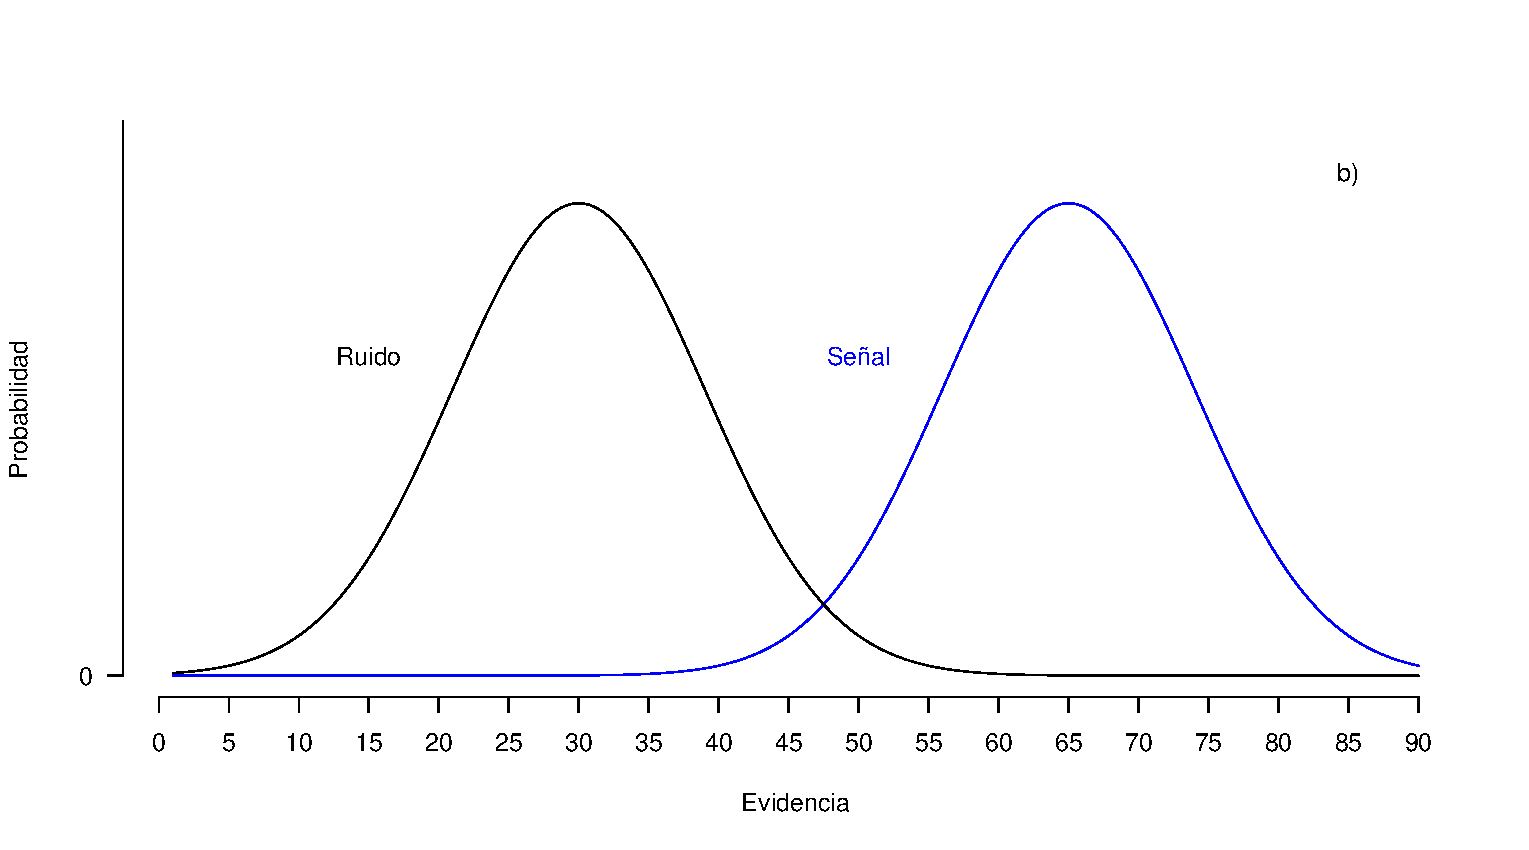
\includegraphics[width=0.55\textwidth]{Figures/Overlap_Small}\\ 
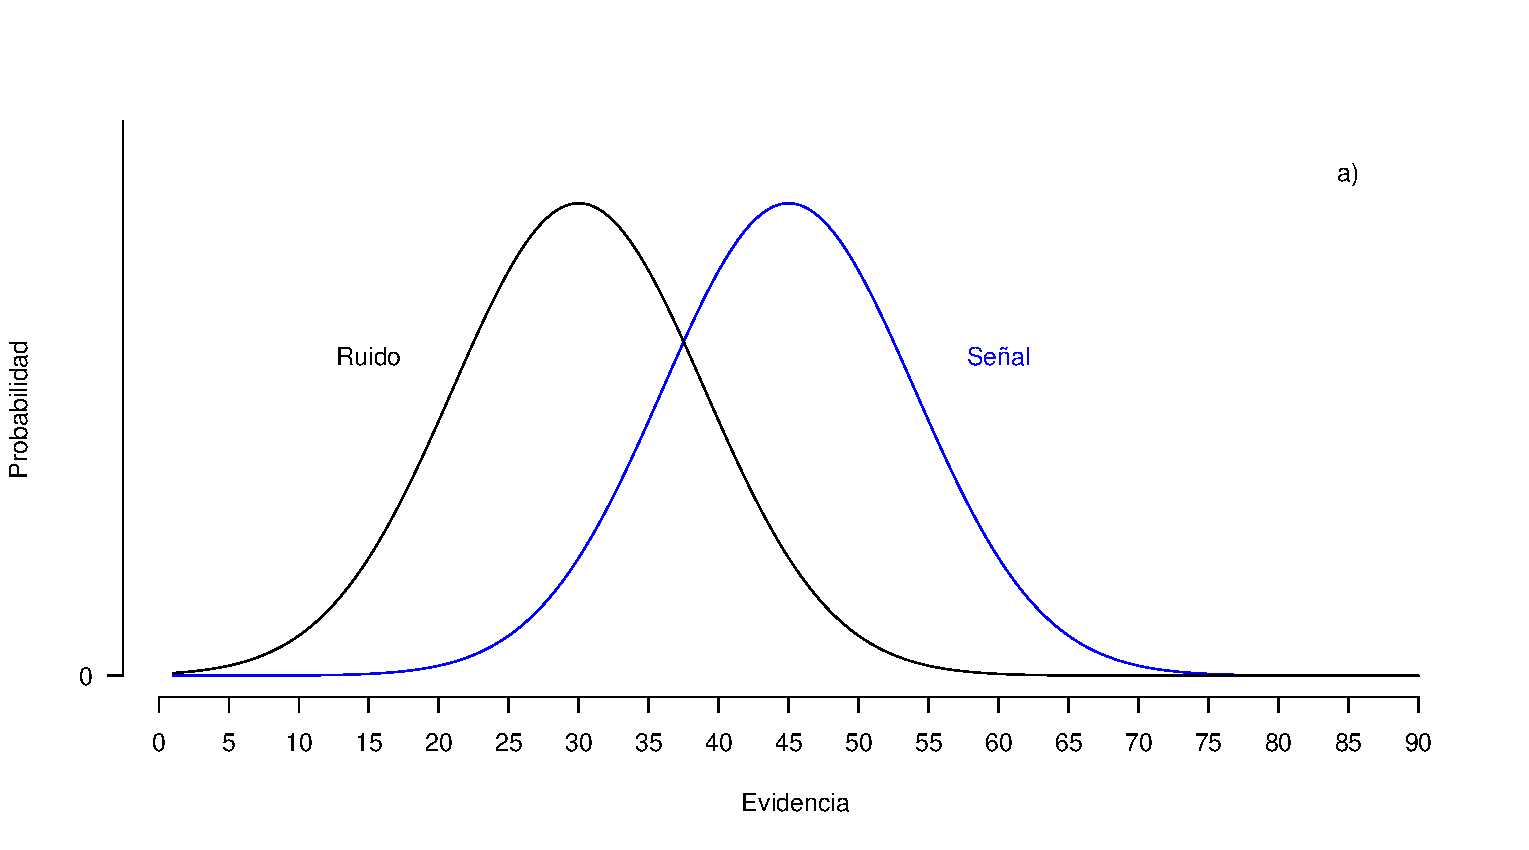
\includegraphics[width=0.55\textwidth]{Figures/Overlap_Big} 
%\decoRule
\caption[El sobrelape Ruido-señal como reflejo de la incertidumbre contenida en tareas de detección]{La distancia entre las distribuciones de ruido y señal determina la incertidumbre contenida en la tarea de detección al variar con ello el área de sobrelape entre las mismas. En el panel a) se presenta un ejemplo donde al estar muy separadas las distribuciones, el sobrelape es pequeño -poca incertidumbre-. En el panel b) se muestra un segundo escenario donde las distribuciones están más cerca, compartiendo más evidencia en el área de sobrelape -más incertidumbre-.}
\label{fig:Overlap}
\end{figure}

La Discriminabilidad en una tarea de detección es producto de la variabilidad con que los posibles estados del mundo se presentan y perciben por los sistemas detectores. Es decir, depende tanto de las propiedades intrínsecas de los estímulos a evaluar -¿qué tanto parecido tienen los estímulos con la señal y los estímulos sin esta?- como de la precisión con que los sistemas detectores son capaces de discernir entre dichas instancias -¿qué tan bueno es el organismo en distinguir una señal del ruido?-. Por ejemplo, no es lo mismo tratar de detectar una manzana entre un montón de naranjas que entre un montón de melocotones y en general, esperaríamos que la tarea fuera más sencilla al tener una mayor discriminabilidad en el primer escenario; así mismo, la tarea de detectar cuando un instrumento musical no está afinado no es igual de difícil para un músico que para una persona sin educación musical.\\

  \textbf{2.- El papel del Sesgo: La detección es decisión}\\

La variabilidad en la presentación y percepción de los posibles estados del entorno -la presencia o ausencia de la señal- constituye el elemento base sobre el cual se desarrolla la TDS y que lleva a concebir la detección de señales como una tarea cargada de incertidumbre, donde los organismos no pueden confiar completamente en la evidencia que se les presenta para emitir un juicio de detección puesto que esta puede relacionarse con cualquiera de las interpretaciones posibles.\\

Los organismos compensan la incertidumbre contenida en las tareas de detección con la información que poseen sobre el entorno. En términos generales, esta puede ser de dos tipos: 1) información probabilística y 2) información sobre las consecuencias comprometidas.\\

Imaginemos por ejemplo el caso de un médico que trata de decidir si los resultados obtenidos en cierta prueba clínica son evidencia suficiente para diagnosticar una enfermedad 'X' a un paciente 'Y'. La evidencia con la que el médico cuenta es imprecisa: toda prueba clínica tiene un margen de error y su lectura debe complementarse con información extraída de su historia clínica. El médico debe juzgar la evidencia en función de toda la información de la que dispone: ¿Qué tan confiable es la prueba?, ¿Cuál es su tasa de aciertos y errores?; ¿Qué tan común es la enfermedad cuya presencia se intenta determinar?, ¿Qué tan probable es que el paciente 'Y' tenga la enfermedad 'X'?; de acuerdo con su historia clínica, ¿qué tanto correlacionan sus características con los factores de riesgo asociados a la enfermedad?, ¿qué tanto cambia la probabilidad de que tenga la enfermedad 'X'?. Y la historia no termina aquí; la información probabilística permite hacer inferencias sobre cuál es la conclusión más probable, pero sigue sin haber certeza sobre el diagnóstico. Para optimizar su comportamiento y tomar la mejor decisión posible, el médico también debe tomar en consideración la información que posee sobre las consecuencias asociadas a cada escenario posible: a) Si el paciente tiene la enfermedad y el médico la detecta acertadamente, podrá tratarse a tiempo; b) Si tiene la enfermedad y el médico falla en detectarla, podría poner en riesgo su vida; c) Si no tiene la enfermedad y el médico le dice que sí, se gastarán recursos innecesarios en solucionar un problema que no existe, corriendo el riesgo de que el tratamiento le haga daño y d) Si no tiene la enfermedad y el médico decide no darle el diagnóstico, todo permanecerá igual. La tarea del médico es mucho más compleja de lo que parecía en un principio, puesto que no se limita a la lectura de una prueba clínica, sino a ponderar lo que sugieren los resultados de la misma con toda la información que posee sobre la probabilidad de las interpretaciones posibles y las consecuencias comprometidas.\\

De acuerdo con la correspondencia entre el estado real del mundo y el juicio emitido por el agente detector, se puede distinguir entre dos tipos de aciertos y errores. Tal y como se muestra en la matriz de contingencia presentada en la Figura~\ref{fig:Mat_Output}, en el marco de la TDS se habla de cuatro posibles resultados: cuando la señal está presente el organismo puede detectarla adecuadamente (Hit) o dejarla pasar (Omisión); a su vez, si la señal no está presente, el organismo puede acertar al diagnosticar su ausencia (Rechazo correcto) o confundir el ruido con la señal, (Falsa Alarma).\\

\begin{figure}[th]
\centering
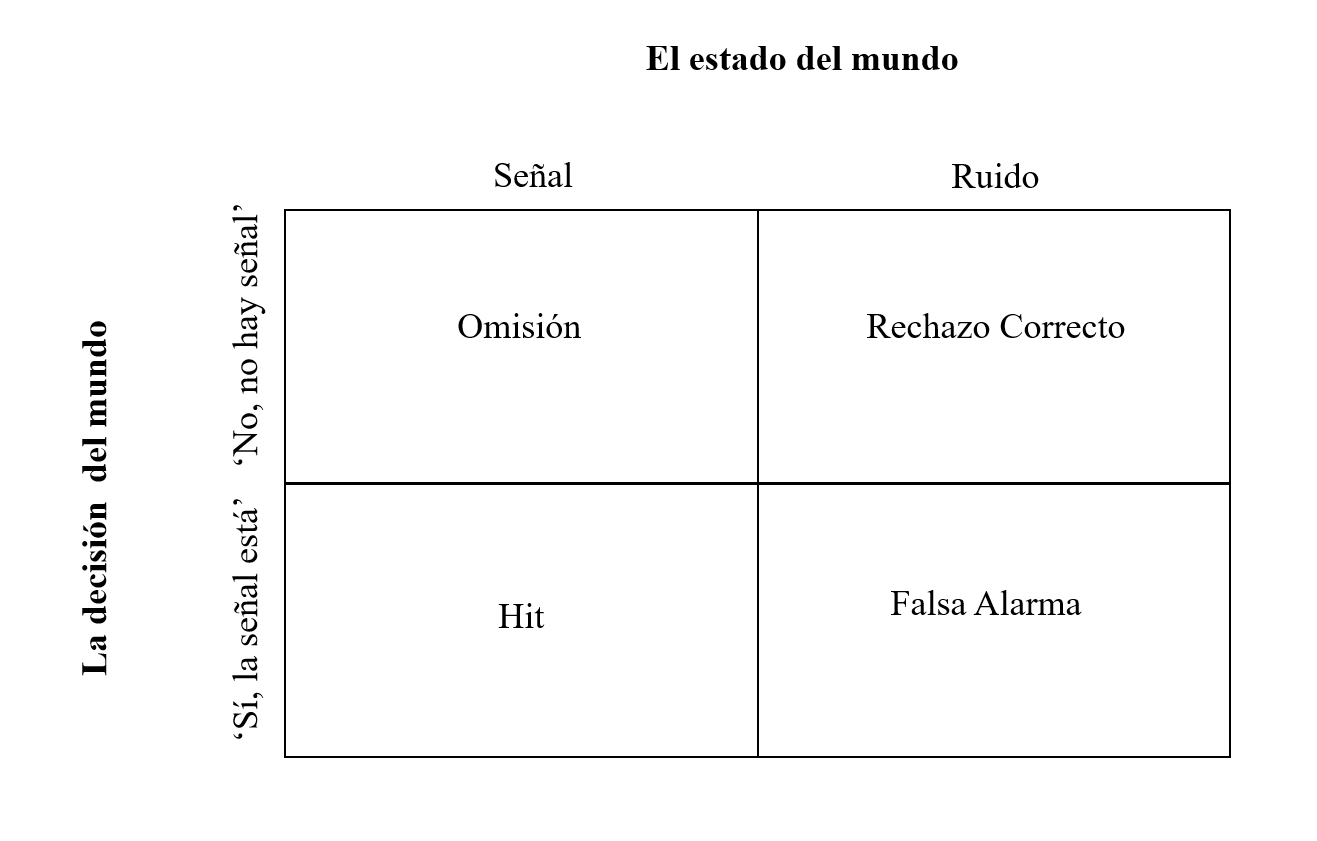
\includegraphics[width=0.60\textwidth]{Figures/Matriz_Outputs} 
%\decoRule
\caption[Posibles Resultados en una Tarea de Detección]{Los cuatro posibles resultados que se espera encontrar de acuerdo con la TDS, dada la incertidumbre contenida en las tareas de detección, en función de la correspondencia que existe entre los juicios emitidos por los organismos y el estado real del mundo.}
\label{fig:Mat_Output}
\end{figure}

La TDS asume que con base en la información de la que dispone sobre la estructura de la tarea, el organismo fija un criterio de elección para determinar a partir de cuánta evidencia va a juzgar la presencia de la señal dado lo que sabe sobre la probabilidad con que ésta ocurre y las consecuencias comprometidas con su detección. En términos de la representación gráfica del modelo, implica que sobre el eje de la Evidencia el organismo sitúa una línea vertical que atraviesa ambas distribuciones y que va a fungir como regla de elección para delimitar a partir de cuánta evidencia  emitir juicios de detección en favor de la señal,como se ilustra en la Figura~\ref{fig:Graf_Outputs} con una línea roja.\\

\begin{figure}[th]
\centering
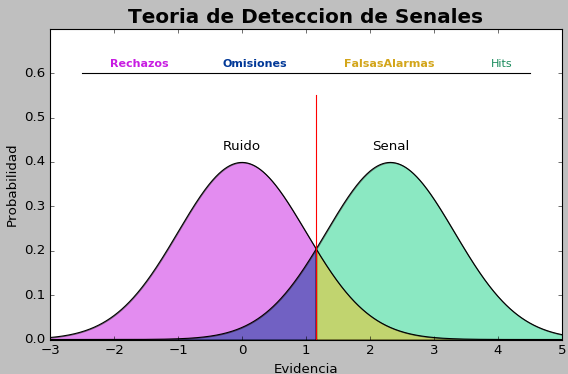
\includegraphics[width=0.60\textwidth]{Figures/Graficador_Tasas} 
%\decoRule
\caption[Posibles Resultados en una Tarea de Detección]{Representación gráfica del problema de detección de señales de acuerdo con la TDS. Existe una distribución de probabilidad que describe las formas en que la señal se presenta en el entorno y una distribución que corresponde a los demás estímulos. Como resultado del traslape entre estas -incertidumbre- el organismo fija un criterio de elección (la línea roja) para determinar a partir de cuánta evidencia juzgará la presencia de la señal, y que determina la probabilidad de obtener cualquiera de los resultados señalados en la figura con distintos colores.}
\label{fig:Graf_Outputs}
\end{figure}

La Figura~\ref{fig:Graf_Outputs} presenta -de forma mucho más completa que las figuras antes mostradas en este capítulo- la forma en que se representan los problemas de detección de señales bajo el marco de la TDS: Se tienen distribuciones de probabilidad que representan la variabilidad con que la señal y el ruido ocurren en el ambiente, y una línea roja que señala el criterio que va a utilizar el agente detector para emitir un juicio de detección. La localización del criterio de elección determina la probabilidad con que, de acuerdo a la cercanía de las distribuciones (discriminabilidad), se esperaría incurrir en cada uno de los cuatro resultados expuestos en la matriz de contingencia de la figura~\ref{fig:Mat_Output}.\\

Dada la estructura de la tarea y el conocimiento que el organismo tenga sobre ella, es posible que se desarrolle una tendencia que favorezca la emisión de un juicio de detección particular. Esto es lo que en el marco de la TDS se identifica como Sesgo. Se asume que la localización del criterio sobre el eje de evidencia es un reflejo del mismo y que su magnitud y dirección depende de dos grandes factores:\\


      \underline{a) Los errores cuestan y los aciertos pagan: Matrices de pago}\\

La variabilidad contenida en la presentación de los estímulos presentes en situaciones de detección da la pauta para que los sistemas inmersos en ellas corran el riesgo de cometer errores.\\

Para entender la importancia en términos de la adaptabilidad de los organismos de las situaciones de detección, es importante recordar que la detección de señales funge como un filtro para orientar su conducta en términos de las consecuencias involucradas. En otras palabras, acertar en un juicio de detección trae consigo ciertas ventajas -derivadas de la adecuada identificación de las reglas operantes en el entorno- y errar cuesta. Y más aún, los distintos tipos de aciertos y errores comprometidos, pagan y castigan en distinta medida.\\

Imaginemos el caso de un animal indefenso -un conejo- que tiene que decidir tan rápido como pueda si el sonido que acaba de escuchar en la maleza corresponde, o no, con el de un depredador. La penalización asociada con cometer una falsa alarma -un gasto innecesario de energía al correr para nada- es sustancialmente diferente a el precio que tendría que pagar por incurrir en una omisión -¡la muerte!-. Dadas las consecuencias en juego, es muy probable que el conejo decida actuar en consecuencia de un juicio de detección afirmativo ("¡Sí, es un depredador!") y correr por su vida, aún ante niveles de evidencia muy bajos.\\

$FALTA AÑADIR MATRIZ DE PAGOS$
\begin{figure}[th]
\centering
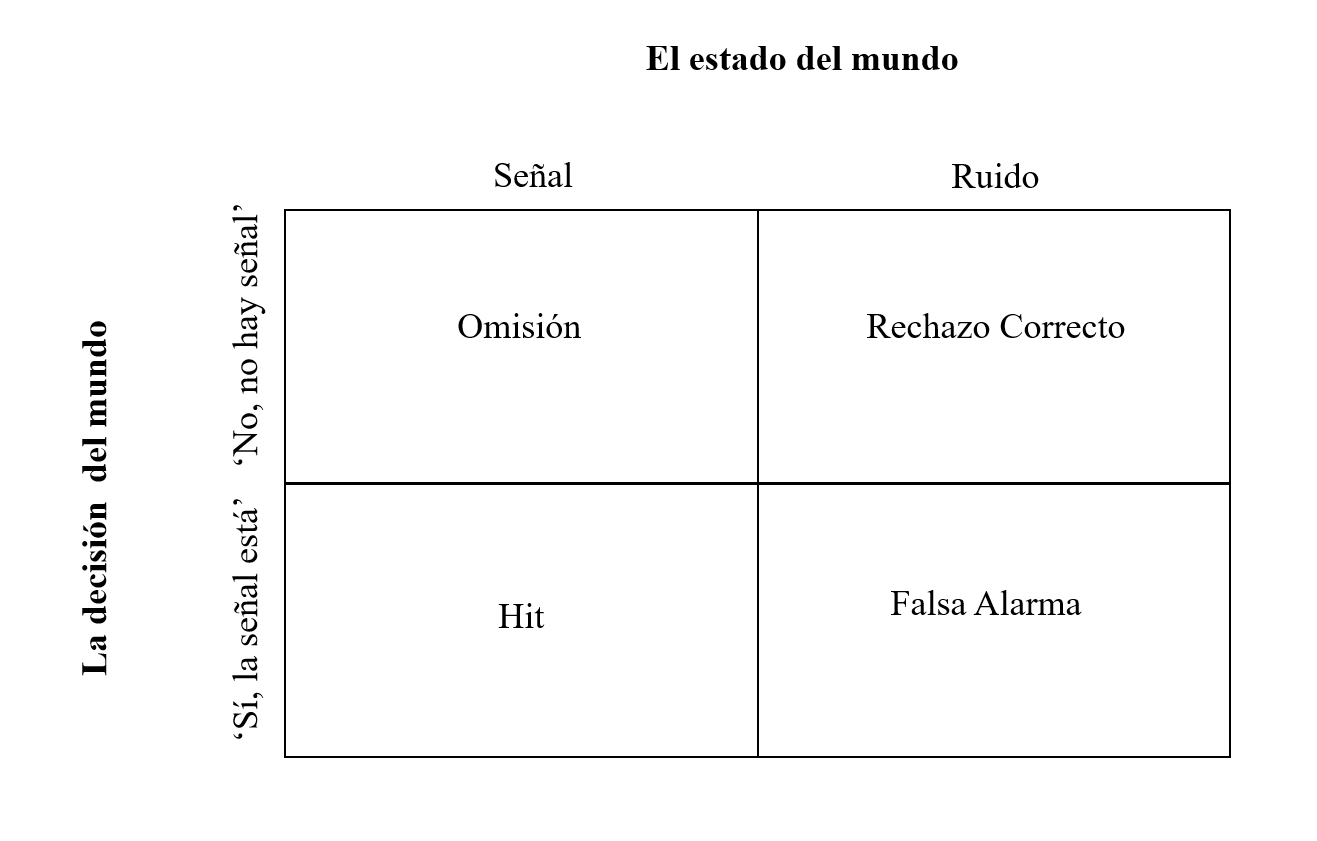
\includegraphics[width=0.60\textwidth]{Figures/Matriz_Outputs} 
%\decoRule
\caption[Ejemplo de Matriz de Pagos]{De acuerdo con el ejemplo planteado en el capítulo acerca de la tarea de detección a la que se enfrenta un conejo que intenta determinar si los sonidos que escucha en su entorno corresponden con los de un depredador, se presenta una matriz de pagos que ilustra los costos y ganancias comprometidos en la tarea en función a la correspondencia entre el juicio elegido y el estado verdadero del mundo.}
\label{fig:Mat_Output}
\end{figure}

La figura~\{} presenta lo que en los modelos clásicos de decisión se conoce como una Matriz de Pagos y que se utiliza para señalar, de acuerdo a una matriz de contingencia, los costos y ganancias asociados con cada resultado observable en tareas de detección $Killeen$. En términos de la TDS, se asume que los organismos toman en cuenta esta información para definir la localización de su criterio de elección. En otras palabras, ya que los organismos nunca podrán tener certeza absoluta sobre los juicios de detección emitidos, se juzga la evidencia a partir de un criterio de elección que toma en cuenta las consecuencias comprometidas en un intento por optimizar su conducta y los resultados obtenidos.\\

      \underline{b) Estimados de Probabilidad}\\

Los organismos involucrados en cualquier tarea de detección tienen alguna expectativa respecto de la probabilidad con que las señales de interés ocurren en el mundo. Es decir, ya sea como resultado de su experiencia directa o porque es información que les ha sido proporcionada de manera externa, los agentes detectores evalúan la evidencia con base en dos grandes probabilidades: 

\begin{itemize}
\item \textsl{Un estimado prior.} Con independencia de cuál sea la evidencia evaluada de manera inmediata, ¿qué tan probable es encontrar la señal en esta situación particular?\\

Si los organismos se encuentran en un entorno donde saben que es prácticamente imposible encontrar la señal, es muy probable que decidan descartar la evidencia que se les presente aún si esta correlaciona con lo que se esperaría de una señal. Por ejemplo, recordemos el ejemplo planteado con anterioridad sobre querer determinar la edad de una persona al hablar con ella por teléfono: si la llamada fue hecha a un despacho de abogados -o cualquier otro escenario donde se piense que es muy poco probable encontrar a un niño-, aún si la persona al otro lado del teléfono tiene una voz muy aguda, es muy poco probable que su interlocutor piense "Oh, estoy hablando con un niño".\\

\item \textsl{La verosimilitud.} Dado lo que se sabe sobre cómo se presentan ciertos estímulos en el entorno -incluyendo la señal-, ¿qué tan verosímil es la evidencia? o bien, ¿qué tan probable exactamente es que la señal o el ruido se presenten con la evidencia que se está evaluando de manera inmediata?\\

Asumir que los organismos apoyan su juicio de detección en el conocimiento que tienen sobre la verosimilitud de la evidencia, es el equivalente a suponer que tienen alguna idea sobre cómo se ven las distribuciones de probabilidad que rigen la ocurrencia del ruido y señal. Bajo este escenario, ante la incertidumbre -si los organismos se enfrentaran a evidencia que cae en el área de sobrelape entre las distribuciones- los agentes detectores optarían por elegir el juicio de detección que corresponda con la distribución que se asocie con dicha evidencia con mayor probabilidad (es decir, la distribución que sea más alta en ese punto particular del eje de decisión).\\
\end{itemize}

De contar con ambos elementos, es posible asumir que los organismos se decantan por un juicio de detección particular con base en el conocimiento que tienen sobre la estructura probabilística del entorno, mediante la realización de una inferencia bayesiana $WEIJIMA$.\\

\subsection{Parámetros del modelo}

Como se mencionó previamente, al realizar una tarea de detección existen dos posibles tipos de aciertos y dos posibles tipos de errores. La materia prima con base en la cual funciona el modelo propuesto por la TDS, son las tasas de aciertos y errores cometidos durante la tarea, de manera que por cada participante que pasa por una tarea de detección, tenemos cuatro tasas que describen su ejecución:

La Tabla 2 ilustra el cómputo de las cuatro tasas de ejecución, como una relación entre el resultado obtenido y el tipo de ensayo con base en el que se le definió como tal. Es decir, tenemos dos tasas definidas en relación al número total de ensayos con la señal (la tasa de hits y la tasa de omisiones) que nos dicen qué proporción de los ensayos con señal fueron detectados correctamente y cuáles se dejaron pasar; y tenemos dos tasas definidas en relación al total de ensayos con ruido (la tasa de falsas alarmas y la tasa de rechazos correctos) que nos describen la relación de los ensayos con ruido que fueron discriminados correctamente y aquellos que se confundieron con la señal.

Para realizar el análisis de datos, bajo el marco de la TDS, sólo necesitaremos un par de estas tasas: la tasa de hits y la tasa de falsas alarmas. Esto bajo el entendido de que las tasas de omisión y rechazos correctos no son más que su complemento, respectivamente, y que estas dos tasas contienen toda la información que necesitamos sobre el desempeño de los participantes.

La idea general de la importancia de estas tasas de ejecución, es que cada una representa el área de las distribuciones de ruido y señal que cae a la izquierda o derecha del criterio de decisión.

Para la estimación paramétrica se utiliza la misma lógica, pero se sigue el procedimiento inverso. Dado que no podemos observar ni cuantificar de manera directa el criterio usado por los participantes para responder a la tarea, qué tan juntas o separadas se encuentran las distribuciones de ruido y señal para cada participante o qué tipo de sesgo pudieran estar siguiendo, utilizamos las tasas de ejecución para hacer inferencias sobre la localización del criterio, la diferencia entre las medias de ambas distribuciones y el grado en que una respuesta se favorece sobre otra. 

A partir de ahora comenzaremos a hablar sobre cómo se calculan cada uno de los parámetros del modelo, de acuerdo a la teoría clásica que sigue los supuestos estadísticos previamente descritos.  Es importante aclarar que el Graficador de Tasas previamente expuesto no representa la teoría con entera precisión; el propósito de ese primer Graficador es simplemente ilustrar cómo describe la TDS el comportamiento de un sistema que se enfrenta ante una tarea de detección, donde existen dos distribuciones que se sobreponen. El Graficador permite manipular directamente la localización del criterio, con la simpleza que implicaría desplazar una línea vertical sobre el eje de decisión y ver qué consecuencias tiene sobre la probabilidad de obtener un tipo particular de acierto o error.


Antes de ahondar a detalle en los parámetros, hay que declarar un par de supuestos formales que hace la Teoría para facilitar la representación gráfica del modelo y la estimación paramétrica:

\begin{enumerate}
\item En su forma clásica, la TDS asume que las distribuciones de ruido y señal son distribuciones normales.
  \begin{itemize}
  \item 
  \end{itemize}
\item En su forma estándar, se asume que las distribuciones de ruido y señal son equivariantes, (compartiendo una desviación estándar de 1).
  \begin{itemize}
  \item 
  \end{itemize}
\item La distribución de ruido tiene su media en 0. 
  \begin{itemize}
  \item La estimación de todos los parámetros del modelo de detección de señales se hace tomando como referencia la distribución del ruido (con  media 0 y desviación estándar de 1)
  \end{itemize}
\end{enumerate}








El soporte de las distribuciones -identificado en la Figura~\ref{fig:Overlap} bajo el nombre de ‘Evidencia’ ( y en las Figuras~\ref{fig:Senal_presentacion} y \ref{fig:Noise}, como 'Puntaje en prueba clínica' e 'Intensidad' en la Figura~\ref{fig:Senal_percepcion}- rara vez se define con precisión,  teniendo una concepción más bien abstracta; La idea general es que cuando queremos detectar una señal particular, comenzamos a recolectar un tipo de evidencia específico a la tarea ante la que nos encontramos. Lo más importante, es que la señal siempre va a estar asociada en mayor medida con dicha evidencia, distribuyéndose siempre en valores situados por encima (a la derecha, en la Figura 1) del ruido.\\
 



Sea cual sea la evidencia con base en la cual se forman los juicios de detección -los valores en el eje X sobre los cuales se despliegan las distribuciones de Ruido y Señal-, se espera que la Señal tenga 'más' de dicha evidencia que el Ruido (en tanto que este último implica su ausencia). 


Por ejemplo, en el caso ilustrado en la Figura~\ref{fig:Noise}, tiene sentido que las personas con Depresión obtengan puntajes más altos dado que la prueba fue hecha para evaluar la presencia de dicha condición y el puntaje final obtenido suele ser reflejo de cuántas de las respuestas proporcionadas coinciden con lo que se esperaría en una persona con Depresión.\\

\begin{itemize}
\item Discriminabilidad $(d')$

La disc

La discriminabilidad se representa en los modelos de detección de señales con un parámetro $d'$, que representa la distancia entre las medias de las distribuciones de ruido y señal. 

Para encontrar la distancia entre las medias de la distribución de ruido y señal, necesitamos saber el punto en que el criterio toca cada distribución. Para ello, calculamos las probabilidades complementarias a las tasas de hits y falsas alarmas y las traducimos a puntajes Z (Ver Fig. 3). Dado que el puntaje Z funciona como una medida de dispersión de la media, basta con restar el puntaje Z de la intersección del criterio con la distribución de señal a el puntaje Z de intersección con la distribución de ruido para conocer la localización de la media de la señal. Por definición, d’ sólo puede tener valores positivos ya que la teoría asume que la distribución de señal siempre está a la derecha de la distribución de ruido porque contiene una mayor cantidad de la evidencia con base en la cual se hace el juicio de detección de la señal.



\item Criterio  $k$

Una vez que hemos resumido el desempeño de nuestro participante en la tarea de detección, el parámetro cuya estimación resulta más sencilla y directa es el Criterio (k). Entender cómo se computa el parámetro nos requiere únicamente de mantener presente el supuesto de que el Ruido se distribuye normalmente y se va a localizar siempre a la izquierda de la señal, por lo que le asignamos una media de cero para tener un punto de referencia para estimar el espacio en que se desarrollan el resto de los parámetros. \\

Para calcular el criterio lo único que necesitamos es conocer la tasa de Falsas Alarmas, que tal y como mencionábamos en el segmento anterior, nos indica qué proporción de la distribución de ruido cae a la derecha del criterio. Dado que a la distribución de ruido, le fue asignada arbitrariamente una media de cero, podemos asignar un valor al punto en que el criterio corta la distribución de ruido y define las tasas de Rechazos y Falsas Alarmas obtenidas por el participante. Conociendo el área de la distribución de Ruido que cae bajo el criterio, (el complemento de la tasa de Falsas Alarmas, o bien, la Tasa de Rechazos correctos), y sabiendo que la distribución tiene una desviación estándar de 1, podemos convertir el valor de la tasa (que corresponde a la probabilidad de cometer un rechazo correcto, de acuerdo al área bajo la curva) en Puntajes Z y conocer la localización del criterio.\\

 El parámetro k, por lo general, va estar representado por un número natural (un número positivo), que indica en términos de Puntajes Z  la posición del criterio sobre el eje de decisión, relativo a la distribución de ruido con media cero. El criterio sólo tiene valores positivos, porque normalmente se espera que la tasa de falsas alarmas nunca tenga un valor mayor a 0.5 (las consecuencias de una tasa de Falsas Alarmas tan alta, se expondrán con más claridad en el apartado correspondiente a la d’. \\


\item Sesgo - $\beta$

El parámetro más comúnmente utilizado en la literatura para evaluar el sesgo de los participantes en estudios donde se aplica el modelo de detección de señales al análisis de tareas experimentales, es Beta ($\beta$). Se define como una razón entre la probabilidad con que la evidencia  \\


distinguiendo entre dos grandes tipos de sesgo: conservador y liberal. 


 El primero favorece la emisión de respuestas negativas al desplazar el criterio a la derecha y requerir al sistema la recolección de mayores niveles de evidencia antes de dar por detectada la señal. El segundo, promueve la detección de la señal, situando el criterio de elección hacia la izquierda, emitiendo un juicio de detección con valores menores de evidencia. Nótese que un sistema carente de sesgo, sería aquel que situara su criterio de elección justo en el punto en que las dos distribuciones se juntan, donde la probabilidad de cometer cualquiera de los tipos de acierto y errores, son iguales entre sí.\\


$\beta = \frac{p(Signal)}{p(Noise)}$

si $\beta<1$ o C<0, sabemos se trata de un sesgo liberal y si $\beta>1$, C>0, hablamos de un sesgo conservador.\\

\item Sesgo - $C$


\end{itemize}   %Terminan los parametros



%----------------------------------------------------------------

\subsection{Tareas de detección}

\begin{itemize}
\item Tareas de detección binaria 

En el laboratorio, la  TDS se estudia a partir  de tareas de detección donde se expone a un  sujeto  a  N  número  de  ensayos,  (comprendidos  por  n  ensayos con  sólo  ruido  y  n  ensayos donde  el  ruido  viene  acompañado  de  la  señal)  ante  los  que  se  le  pide  al  participante  que responda eligiendo una de dos opciones: Sí está la señal o No está la señal. En estos escenarios controlados,  el  experimentador  decide  la  proporción  de  ensayos  con  y  sin  señal  que  se presentarán, así como la matriz de pagos que definirán la utilidad de sus aciertos y errores. \\


\item Tareas con escala de confianza

Un segundo procedimiento comúnmente utilizado en tareas de detección implica añadir un paso adicional a la tarea de los participantes. 

\parencite{McNicol}

\item Tarea con elección forzada entre dos alternativas.



\end{itemize}














\section{Panorama general del estudio de Memoria de Reconocimiento}

\subsection{Teoría del Umbral}

%-----------------------------------
%	SUBSECTION 1
%-----------------------------------
\subsection{Teoría del Procesamiento Dual}

La Teoría del Procesamiento Dual (TPD; o PDT por sus siglas en inglés) sostiene que existen dos procesos fundamentales involucrados en todo juicio de reconocimiento: la recolección y el análisis de familiaridad. El primero corresponde a la extracción de rasgos y detalles específicos del estímulo a evaluar, (i.e. el estímulo que queremos determinar si se ha visto antes, o no), un proceso que requiere cierto tiempo; el segundo, es entendido como un fenómeno más o menos automático y casi instantáneo donde el sistema identifica el estímulo como 'familiar' y decide que lo ha reconocido de alguna experiencia previa. 

%-----------------------------------
%	SUBSECTION 2
%-----------------------------------

\section{Teoría de Detección de Señales en Memoria de Reconocimiento}
Aplicar la TDS al estudio de la Memoria de Reconocimiento implica asumir que existe tal cosa como una 'fuerza de memoria' ('memory strength', en inglés) que refleja el grado en que un estímulo cualquiera es percibido como 'familiar' para el sistema que busca emitir un juicio de detección. La fuerza de memoria evocada por cada estímulo se compara con un criterio de elección para que el sistema pueda decidir si lo reconoce, o no, como 'elemento antes visto'.\\ 

\begin{figure}[th]
\centering
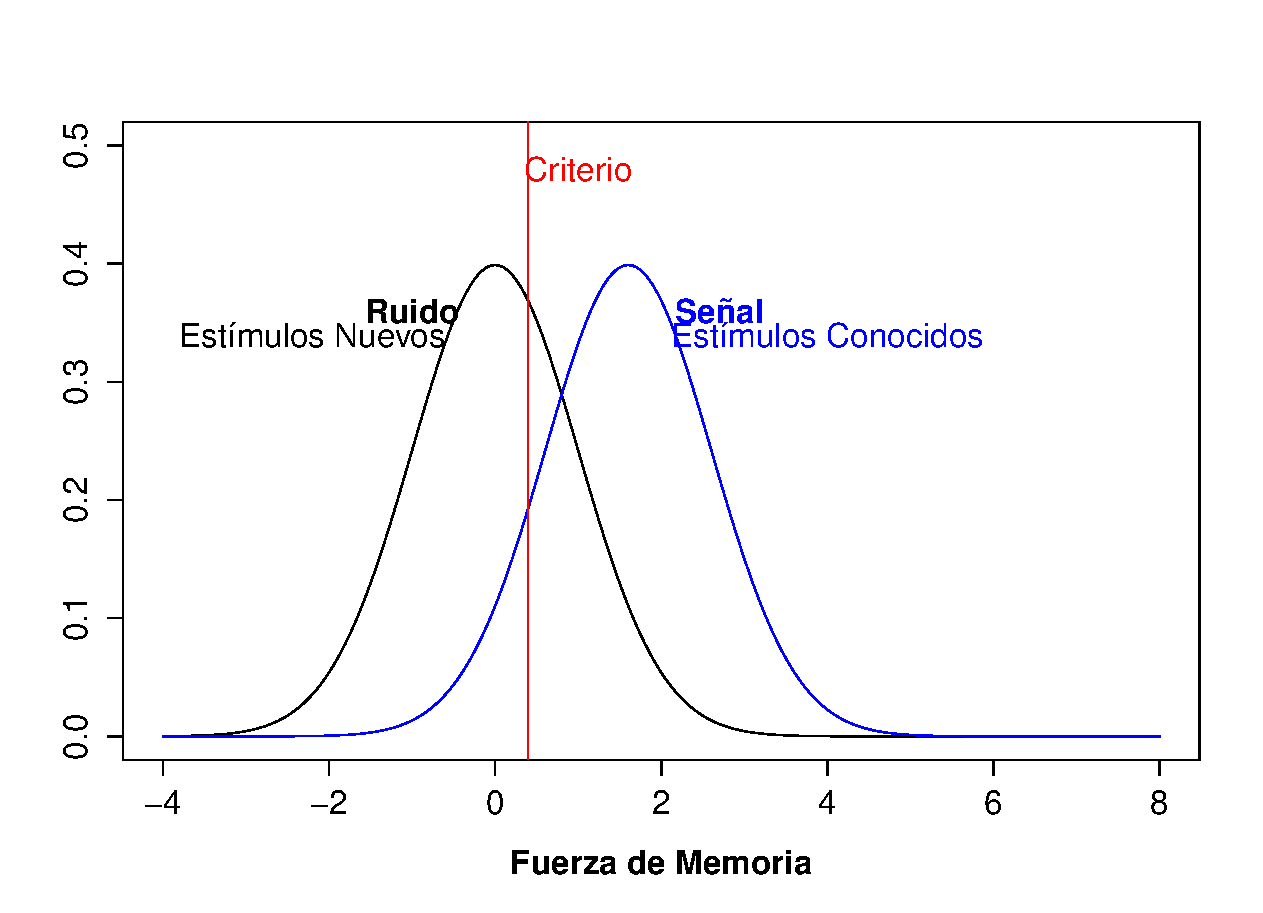
\includegraphics[width=0.60\textwidth]{Figures/RM_SDT_1} 
\decoRule
\caption[SDT en Memoria de Reconocimiento]{Modelo de Detección de Señales aplicado al estudio de Memoria de Reconocimiento}
\label{fig:RM_SDT_1}
\end{figure}

La Figura~\ref{fig:RM_SDT_1} ilustra la forma en que los supuestos de la TDS, expuestos a detalle en el Capítulo 1, se aplican al estudio de la Memoria de Reconocimiento. Las idea central se mantiene en escencia y simplemente sustituimos algunos conceptos: al tratarse de una tarea de reconocimiento, decimos que la 'señal' a detectar es cualquier estímulo antes visto (i.e. 'estímulos viejos', como suelen identificarse en la literatura); el 'ruido' son los estímulos nuevos, que podrían -o no- confundirse con los primeros; el 'eje de decisión' a lo largo del cual se sitúan las dos distribuciones de ruido y señal, se convierte en un 'eje de familiaridad' que va a representar distintos grados de lo que parece ser una 'fuerza de memoria'. También se mantienen las ideas centrales propuestas por el modelo: los estímulos ya antes vistos tendrán valores más altos de 'familiaridad' que aquellos nunca antes vistos, admitiendo sin embargo la posibilidad de que éstos últimos puedan llegar a confundirse con los estímulos viejos, por ejemplo, si comparten algun rasgo en particular; una vez más, dicha variabilidad en la presentación y lectura de los estímulos a evaluar se refleja en la idea de que existen distintos rangos de familiaridad que pueden ser producidos por los estímulos viejos o conocidos, con cierta distribución de probabilidad. Y de la misma forma, la emisión de un juicio se entiende como resultado de comparar la 'familiaridad' de cada estímulo a evaluar con un criterio de elección particular, donde sólo si éste se rebasa, se juzga el estímulo como 'ya antes visto'.\\

Como se mencionó en el Capítulo 1, la TDS en su forma típica define las distribuciones de ruido y señal como distribuciones Gaussianas con varianzas iguales (i.e. con una misma desviación estándar). A propósito de ello, podemos hablar de una particularidad que tiene la aplicaicón de la TDS a estudios de memoria de reconocimiento, que ha sido constante y consistentemente demostrada con los datos: la distribución de Estímulos Viejos suele mostrar mayor desviación estándar que la distribución de Ruido, justo como se muestra en la Figura~\ref{fig:RM_SDT_2}.\\


\begin{figure}[th]
\centering
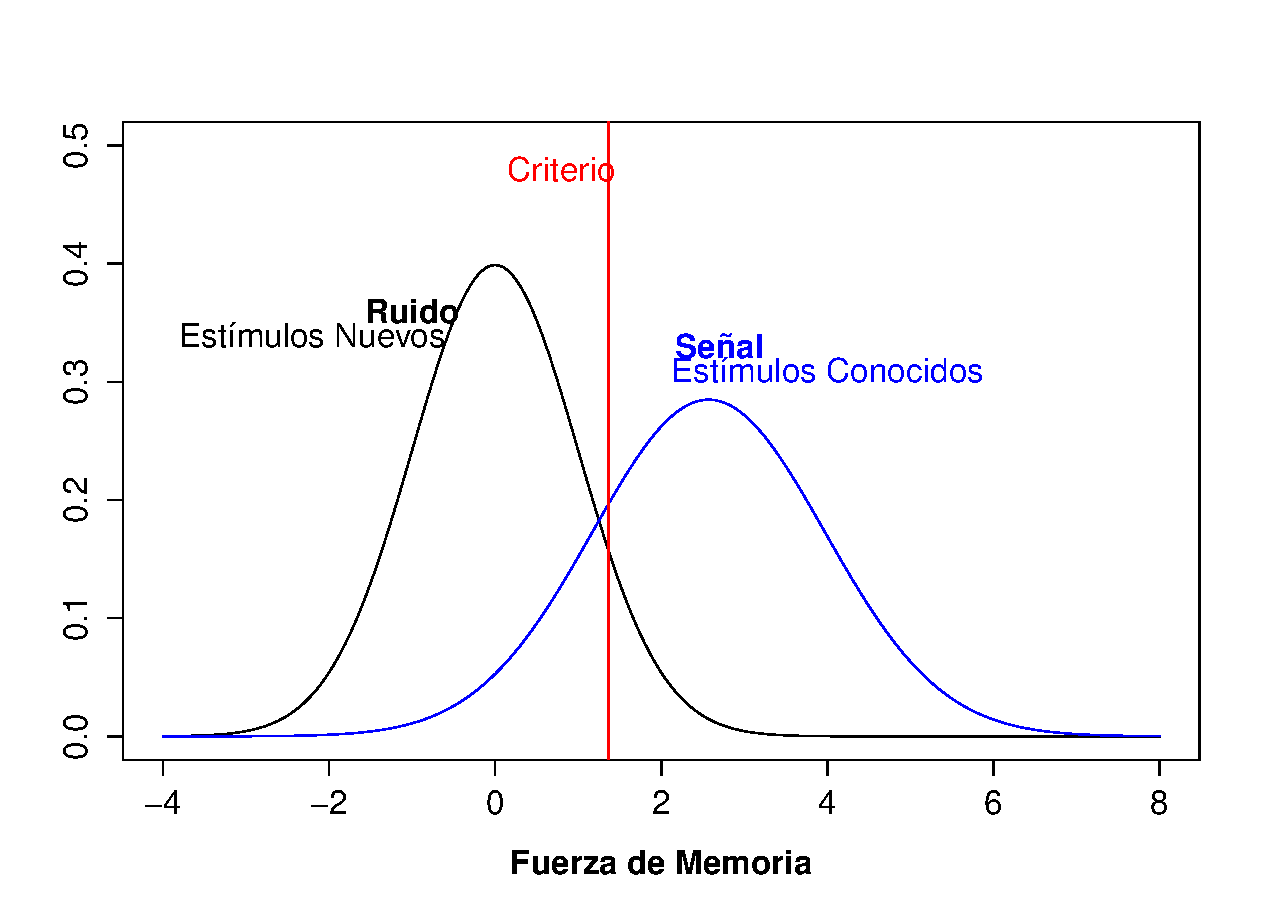
\includegraphics[width=0.60\textwidth]{Figures/RM_SDT_2} 
\decoRule
\caption[SDT en Memoria de Reconocimiento (Varianzas Desiguales)]{Modelo de Detección de Señales con varianzas desiguales aplicado al estudio de Memoria de Reconocimiento}
\label{fig:RM_SDT_2}
\end{figure}


\subsection{Implicaciones y conflictos}

Me permitiré, por un momento, salirme del molde académico y hablar un poco de todo el proceso que hubo detrás de la realización del presente trabajo. Cuando comencé a revisar literatura para decidir cuál podría ser mi proyecto de tesis, descubrí la maravilla de la Teoría de Detección de Señales. 

Sin embargo, pese a la flexibilidad de la que dispone la TDS para aplicarse a, aparentemente, cualquier tarea de decisión binaria, donde se admita el papel de la incertidumbre en la emisión de un juicio de detección, su aplicación al campo de la Memoria de Reconocimiento no ha estado excenta de críticas.

Conceptualmente, es fácil pensar en una tarea de reconocimiento en términos del modelo de detección de señales. Sin embargo, cuando se revisan las implicaciones teóricas que conllevaría aceptar que la memoria de Reconocimiento funciona como un procedimiento cualquiera de detección de señales, no son del todo claras. 

\section{El Efecto Espejo}

“is usually interpreted in terms of (unequal variance) signal detection theory (SD) in which case it implies that the order of the underlying old item distributions mirrors the order of the new item distributions” (DeCarlo, L.,  2007)\\
Teoría de Atención /Verosimilitud: Un modelo de marcaje de rasgos, determinado por un muestreo diferencial dada la condición (H-frequency, L-frequency)\\
Teoría de Atención / Verosimilitud; demasiado complicada, sus supuestos no son necesarios (Decarlo, 2007; Hintzman, 1994; Murdock, 1998) Intercambio de papers Hintzman-Glanzer\\
‘The mixture model’ (DeCarlo, 2007) – Extensión de la SDT, una extensión mezclada.\\
Between vs Within condition discussion (Listas separadas o mezcladas)\\
Between condition: Problemas (1) No se puede descartar la posibilidad de que el criterio de respuesta difiera a lo largo de las condiciones. Y (2) las distribuciones subyacentes no necesariamente están escaladas de la misma forma a lo largo de las dos condiciones.\\
“one cannot compare the values of d’ across the two conditions without further assuming that the variance of the reference distributions (LN and HN) are the same, which does not appear to be the case. (DeCarlo,2007)  

%----------------------------------------------------------------------------------------
%	SECTION 1
%----------------------------------------------------------------------------------------

\subsection{Evidencia recolectada}

Teóricamente, este procedimiento nos permitiría inferir no uno, sino seis sub-criterios de elección que estarían permeando a partir de cuánta evidencia el participante se siente más, o menos seguro, de si los estímulos evaluados contienen la señal o sólo ruido. De encontrarse evidencia del Efecto Espejo en los experimentos realizados, se esperaría encontrar el mismo patrón en el promedio de los puntajes de confianza asignados a cada una de las cuatro categorías de estímulos (formadas por la combinación Condición (A o B) x Tipo de ensayo (S o R)) reportados en la literatura en Memoria de Reconocimiento \parencite{Glanzer1990, Glanzer1993}. \\

La Figura~\ref{fig:Ejem_Crit} 

\begin{figure}[th]
\centering
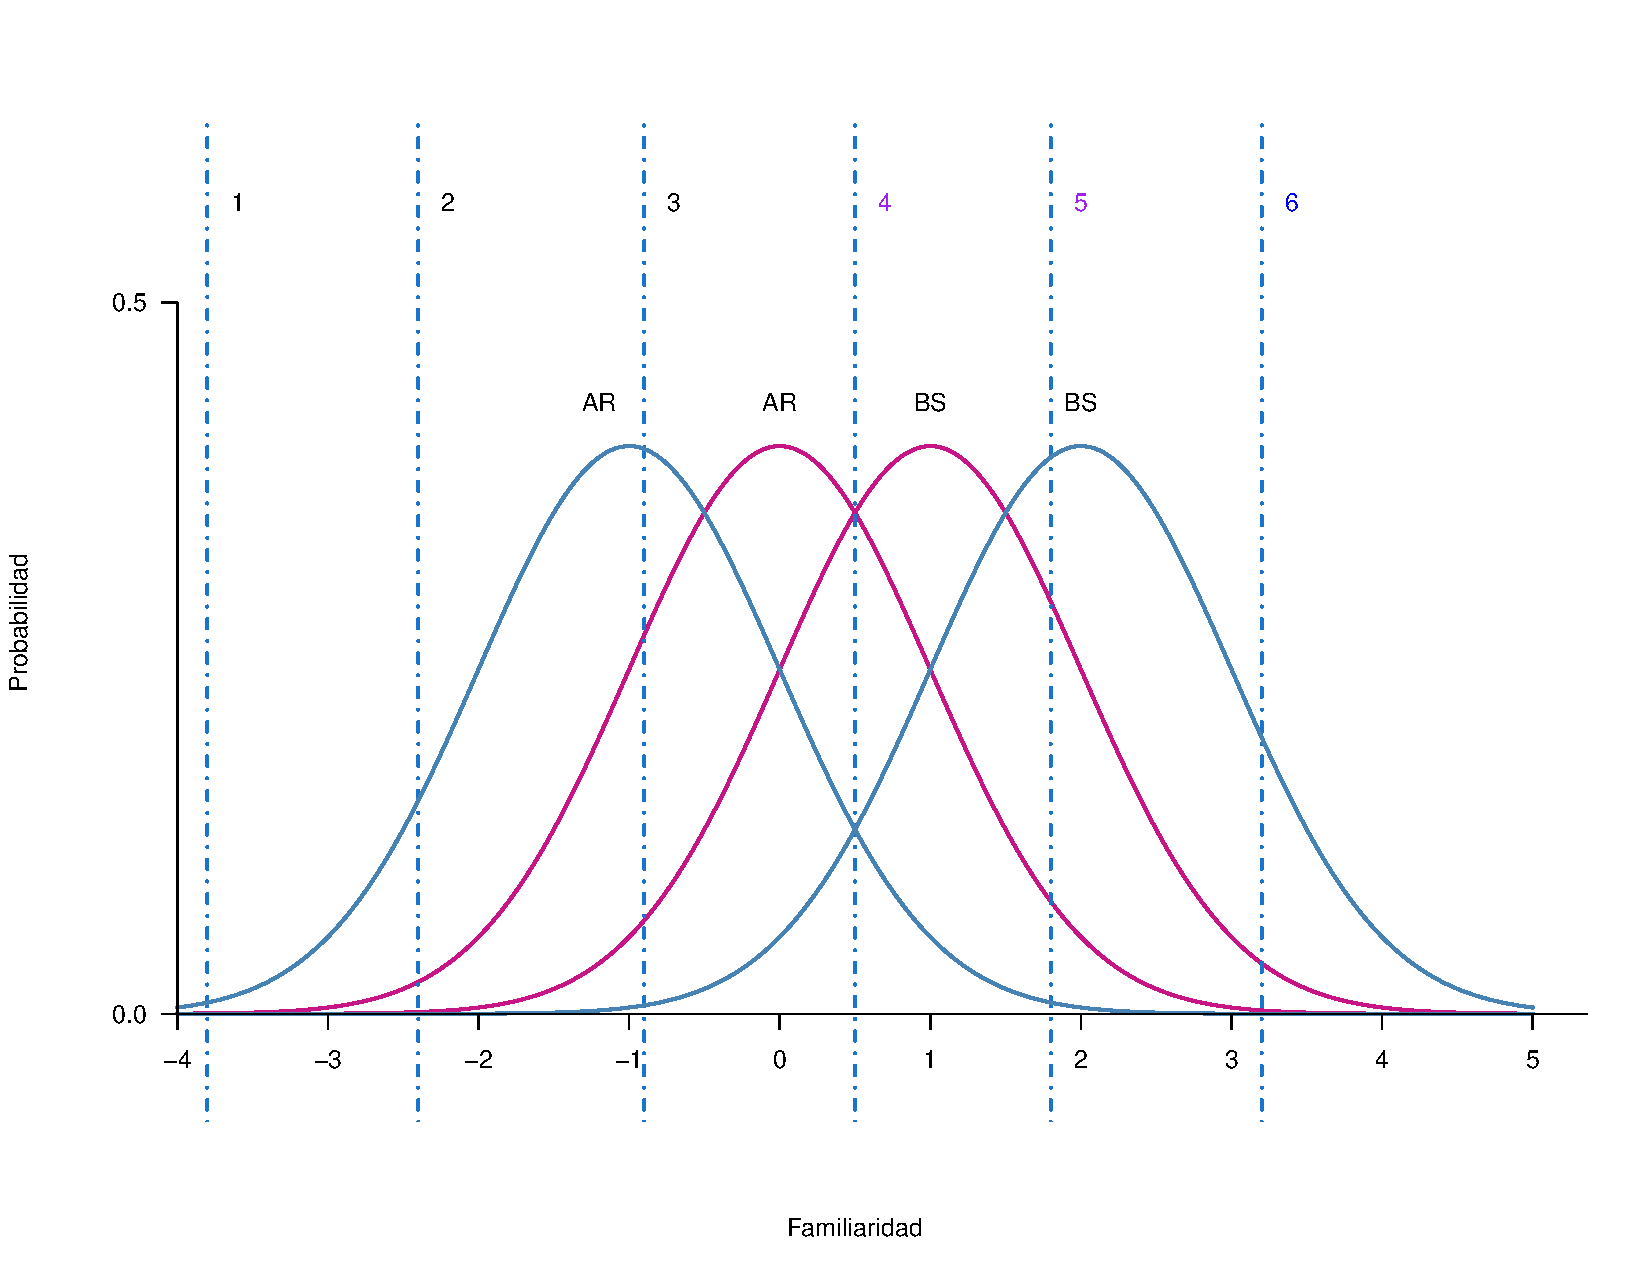
\includegraphics[width=0.55\textwidth]{Figures/Ejem_Criterios}
%\decoRule
\caption[Representación gráfica de los sub-Criterios para la emisión de puntajes de confianza ]{}
\label{fig:Ejem_Crit}
\end{figure}



\subsection{Relevancia e implicaciones}
A primera vista el patrón de respuestas identificado como Efecto Espejo podría parecer trivial: Si sabemos que lo que distingue a las condiciones de estímulos 

%-----------------------------------
%	SUBSECTION 1
%-----------------------------------
\subsection{Algunos modelos desarrollados para dar cuenta del Efecto Espejo}

\begin{itemize} 
\item
\item
\end{itemize}


